\chapter{Пошук карти глибин за спереопарою}

Другий розділ присвячено розв'язку задачі стереобачення алгоритмом дифузії.
Описуються властивості алгоритму та з'ясовується придатність
розв'язку для поставленої задачі.

\section{Відомості з теорії оптимізації}
Введемо декілька визначень \cite{overview:savchynskyy:diffusion},
що знадобляться при розв'язанні задачі.

Нехай задача
\begin{equation} \label{minimization:problem}
    \min_{\pmb{x} \in X} f \left( \pmb{x} \right)
\end{equation}
є задачею мінімізації функції $f: X \to \mathbb{R}$ на множині
$X \subseteq \mathbb{R}^n$.
Тоді оптимізаційна задача
\begin{equation*}
    \min_{\pmb{x} \in X'} g \left(\pmb{x} \right)
\end{equation*}
називається релаксацією задачі \eqref{minimization:problem},
якщо $X' \supseteq X$ та $g \left( \pmb{x} \right) \ge f \left( \pmb{x} \right)$
для будь-якого $\pmb{x} \in X$.

Опуклим бакатогранником (polyhedron) $P$ в $\mathbb{R}^n$ називається множина,
що може бути представлена скінченним набором лінійних нерівностей,
тобто
$P = \left\{
    \pmb{x} \in \mathbb{R}^n \; \middle| \;
    \hat{A} \cdot \pmb{x} \le \pmb{b}
\right\}$
для матриці $\hat{A} \in \mathbb{R}^{m \times n}$ і вектору
$\pmb{b} \in \mathbb{R}^n$.
Обмежений опуклий багатогранник називається політопом (polytope).

Політоп
\begin{equation*}
    \Delta^n := \left\{
        \pmb{x} \in \mathbb{R}^n_+ \; \middle| \; \sum \limits_{x = 1}^n x_i = 1
    \right\}
\end{equation*}
називається $n$-вимірним (ймовірнісним) симплексом.

Нехай $P$~---~опуклий багатогранник в $\mathbb{R}^n$,
визначений множиною лінійних обмежень.
Оптимізаційні задачі виду
\begin{equation*}
    \min \limits_{\pmb{x} \in P} \langle \pmb{c}, \pmb{x} \rangle, \qquad
    \max \limits_{\pmb{x} \in P} \langle \pmb{c}, \pmb{x} \rangle
\end{equation*}
називаються задачами лінійного програмування

Задача лінійного програмування з додатковим обмеженням,
яке дозволяє всім змінним приймати значення тільки $0$ або $1$,
наприклад,
\begin{equation*}
    \min \limits_{\pmb{x} \in P \cap \left\{ 0, 1 \right\}}
    \langle \pmb{c}, \pmb{x} \rangle,
\end{equation*}
називається задачею булевого цілочисельного лінійного програмування.

Розглянемо задачу цілочисельного лінійного програмування
\begin{equation} \label{ILP}
    \min \limits_{\substack{\pmb{x} \in P \cap \left\{ 0, 1\right\}^n \\
                  \hat{A} \cdot \pmb{x} = \pmb{b}}}
        \langle \pmb{c}, \pmb{x} \rangle,
\end{equation}
де $P$~---~політоп, $\hat{A} \in \mathbb{R}^{m \times n}$,
$\pmb{b} \in \mathbb{R}^n$.
Дуальна функція Лагранжа для задачі \eqref{ILP} має вигляд
\begin{equation} \label{dualization}
    \min \limits_{\pmb{x} \in P \cap \left\{ 0, 1 \right\}^n}
        \langle \pmb{c}, \pmb{x} \rangle +
    \langle \lambda, \hat{A} \cdot \pmb{x} - \pmb{b} \rangle, \qquad
    \lambda \in \mathbb{R}^n.
\end{equation}
Змінна $\pmb{\lambda}$ називається дуальною змінною.
Цей прийом називається дуалізацією обмежень $\hat{A} \cdot \pmb{x} = \pmb{b}$,
а релаксації такого вигляду називаються лагранжевими релаксаціями.
Наступна задача є дуальною задачею Лагранжа для задачі \eqref{ILP}
\begin{equation*}
    \max \limits_{\lambda \in \mathbb{R}^n}
        \min \limits_{\pmb{x} \in P \cap \left\{ 0, 1 \right\}^n}
            \langle \pmb{c}, \pmb{x} \rangle +
        \langle \lambda, \hat{A} \cdot \pmb{x} - \pmb{b} \rangle.
\end{equation*}

\section{Релаксація Лагранжа для поставленої оптимізаційної задачі}

Введемо вектор $\pmb{\mu}$, який містить змінну з множини $ \left[ 0, 1 \right]$
для кожної вершини
$\left( x, y, d \right), \left(x, y \right) \in T, d \in D$ та кожної дужки
$\left( \left( x, y, d \right), \left(x', y', d' \right) \right)$,
що поєднує пари міток $d, d' \in D$ між сусідніми об'єктами
$\left(\left(x, y \right), \left(x', y' \right) \right) \in \mathcal{N}$
в побудованому графі.
Множину всіх вершин і дужок графу позначимо через $\mathcal{I}$.

Елементи даного вектору $\mu_{\left(x, y \right)} \left(d \right)$,
що відповідають вершинам, мають бути узгодженими з розміткою $\pmb{d}$,
тобто якщо $\mu_{\left(x, y \right)} \left(d^* \right) = 1$ для якоїсь мітки
$d^* \in D$,
то $d \left(x, y \right) = d^*$.
Розмітка $\pmb{d}$, за визначенням,
має в кожному об'єкті $\left(x, y \right) \in T$
обрати одну й тільки одну мітку $d \in D$.
Таким чином, на елементи вектора $\pmb{\mu}$
накладаються обмеження однозначності для вершин в об'єкті
\begin{equation} \label{vetrex:unambiguity}
    \sum \limits_{d \in D} \mu_{\left( x, y \right)} \left( d \right) = 1,
    \qquad \forall \left(x, y \right) \in T,
\end{equation}
тобто у випадку, якщо вектор $\pmb{\mu}$~---~бінарний,
то тільки один його елемент,
що відповідає вершинам в об'єкті $\left(x, y \right)$, може бути рівним одиниці.

Якщо в об'єкті обрана вершина $d^*$, то обрані дужки,
що виходять із даного об'єкту до сусідніх об'єктів,
мають виходити з цієї ж вершини (рис.~\ref{fig:combining:constraints}).
Ці обмеження називаються поєднуючими
\begin{equation} \label{combining:constraints}
    \sum \limits_{d \in D}
        \mu_{\left(x, y \right), \left(x', y' \right)} \left(d, d' \right) =
        \mu_{\left(x', y' \right)} \left(d' \right), \qquad
    \forall
    \left( \left(x, y \right), \left(x',y' \right) \right) \in \mathcal{N},
    d' \in D.
\end{equation}

\begin{figure}[h]
  \centering
  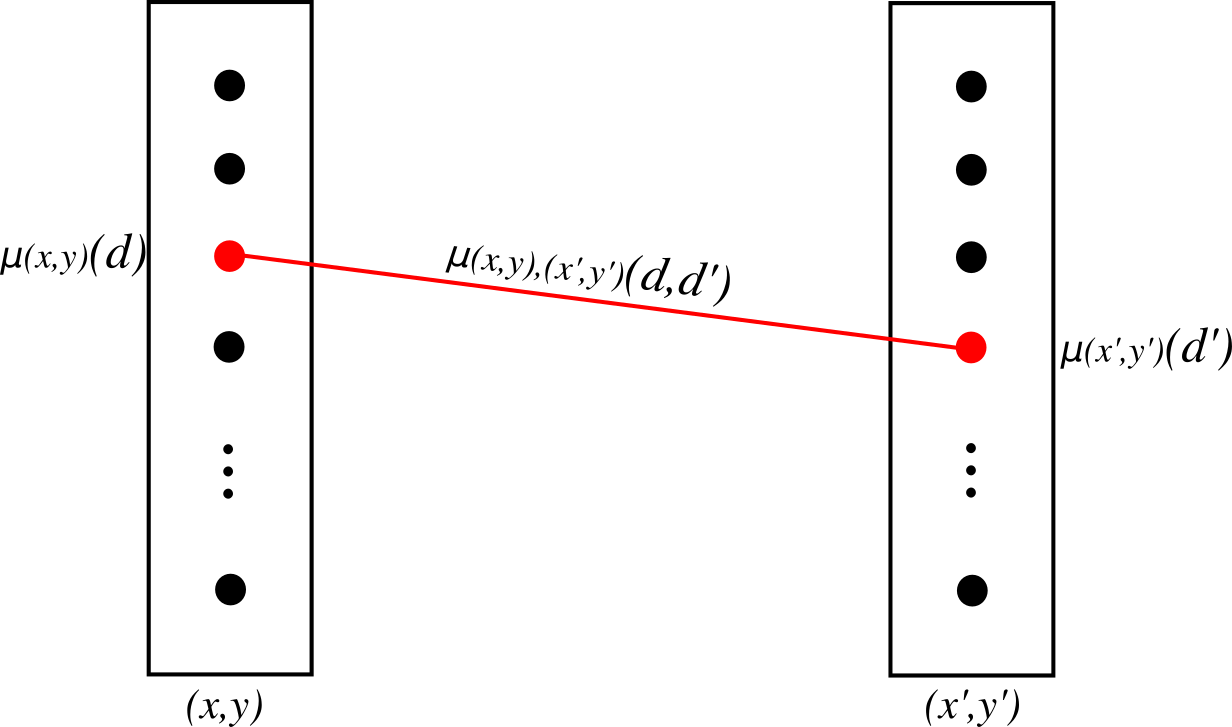
\includegraphics[width=0.7\textwidth]{images/combining_constraints}
  \caption{Поєднуючі обмеження}
  \label{fig:combining:constraints}
\end{figure}

З цих обмежень також випливає,
що між двома сусідніми об'єктами може бути обрана лише одна дужка,
тобто на вектор $\pmb{\mu}$
ще накладаються обмеження однозначності для дужок між парами сусідніх об'єктів
\begin{equation} \label{edge:unambiguity}
    \sum \limits_{d, d' \in D}
        \mu_{\left(x, y \right), \left(x', y' \right)} \left(d, d' \right) = 1,
        \qquad \forall
        \left(\left(x, y \right), \left(x', y' \right) \right) \in \mathcal{N}.
\end{equation}

Обмеження \eqref{vetrex:unambiguity}, \eqref{combining:constraints} та
\eqref{edge:unambiguity} утворюють локальний політоп
\begin{equation} \label{local:polytop}
\begin{gathered}
    \mathcal{L} :=
    \begin{cases}
        \sum \limits_{d \in D}
            \mu_{\left(x, y \right), \left(x', y' \right)} \left(d, d' \right) =
            \mu_{\left(x', y' \right)} \left(d' \right), \;
        \forall
        \left( \left(x, y \right), \left(x',y' \right) \right) \in \mathcal{N},
        d' \in D, \\
        \sum \limits_{d \in D} \mu_{\left( x, y \right)} \left( d \right) = 1,
        \qquad \forall \left(x, y \right) \in T, \\
        \sum \limits_{d, d' \in D}
            \mu_{\left(x, y \right), \left(x', y' \right)} \left(
                d, d'
            \right) = 1, \qquad \forall
            \left(\left(x, y \right), \left(x', y' \right) \right) \in
                \mathcal{N}, \\
        \pmb{\mu} \ge \pmb{0},
    \end{cases}
\end{gathered}
\end{equation}
де остання нерівність означає, що кожен елемент вектора $\pmb{\mu}$ невід'ємний.

Отримаємо задачу цілочисельного лінійного програмування
\begin{equation*}
    \min \limits_{\pmb{d} \in D^T} E \left( \pmb{d} \right) =
    \min \limits_{\pmb{\mu} \in \mathcal{L} \cap \left\{ 0, 1 \right\}^{\mathcal{I}}}
        \langle \pmb{\theta}, \pmb{\mu} \rangle,
\end{equation*}
де $\pmb{\theta}$~---~вектор штрафів, накладених на всі вершини та дуги,
елементи якого розташовані в тій же послідовності,
що й елементи вектора $\pmb{\mu}$.

Випишемо скалярний добуток у правій частині останнього виразу в явному вигляді
\begin{equation} \label{ILP:MAP:inference}
\begin{gathered}
    \min \limits_{\pmb{\mu} \in \mathcal{L} \cap \left\{ 0, 1 \right\}^{\mathcal{I}}}
        \langle \pmb{\theta}, \pmb{\mu} \rangle =
    \min \limits_{\pmb{\mu} \in \mathcal{L} \cap \left\{ 0, 1 \right\}^{\mathcal{I}}}
        \left[
            \sum \limits_{\left(x, y \right) \in T}
                \sum \limits_{d \in D}
                    \mu_{\left(x, y \right)} \left(d \right) \cdot
                    f_{\left(x, y \right)} \left( d \right) + \right. \\
            + \left.
            \sum \limits_{\left(\left(x, y \right), \left(x', y' \right) \right) \in \mathcal{N}}
                \sum \limits_{d, d' \in D}
                    \mu_{\left(x, y \right), \left(x', y' \right)} \left(
                        d, d'
                    \right) \cdot
                    g_{\left(x, y \right), \left(x', y' \right)} \left(
                        d, d'
                    \right)
        \right].
\end{gathered}
\end{equation}

Використаємо прийом дуалізації \eqref{dualization}
поєднуючих обмежень \eqref{combining:constraints}
в задачі \eqref{ILP:MAP:inference}.
Новий доданок має вигляд
\begin{equation} \label{dualized:term}
    \sum \limits_{\left(x, y \right) \in T}
        \sum \limits_{\left(x', y' \right) \in \mathcal{N} \left(x, y \right)}
            \sum \limits_{d \in D}
                \varphi_{\left(x, y \right), \left(x', y' \right)} \left(
                    d
                \right) \cdot \left[
                    \sum \limits_{d' \in D}
                        \mu_{\left(x, y \right), \left(x', y' \right)} \left(
                            d, d'
                        \right) - \mu_{\left(x, y \right)} \left(d \right)
                \right],
\end{equation}
де змінні
$\varphi_{\left(x, y \right), \left(x', y' \right)} \left( d \right) \in
    \mathbb{R}$,
$\left(x, y \right) \in T$,
$\left(x', y' \right) \in \mathcal{N} \left(x, y \right)$,
$d \in D$,
є дуальними.
Будемо називати їх потенціалами (рис.~\ref{fig:phi:block}).

\begin{figure}[h]
  \centering
  \includegraphics[width=0.6\textwidth]{images/phi_block}
  \caption{Змінна $\varphi_{\left(x, y \right), \left(x', y' \right)} \left(d \right)$}
  \label{fig:phi:block}
\end{figure}

Запишемо цільову функцію задачі \eqref{ILP:MAP:inference}
з урахуванням нового доданку \eqref{dualized:term}, в якому розкриємо дужки
\begin{equation*}
\begin{gathered}
    \langle \pmb{\theta}^{\varphi}, \pmb{\mu} \rangle =
    \sum \limits_{\left(x, y \right) \in T}
        \sum \limits_{d \in D}
            \mu_{\left(x, y \right)} \left(d \right) \cdot
            f_{\left(x, y \right)} \left( d \right) + \\
    + \sum \limits_{\left(\left(x, y \right), \left(x', y' \right) \right) \in \mathcal{N}}
        \sum \limits_{d, d' \in D}
            \mu_{\left(x, y \right), \left(x', y' \right)} \left(
                d, d'
            \right) \cdot
            g_{\left(x, y \right), \left(x', y' \right)} \left(
                d, d'
            \right) + \\
    + \sum \limits_{\left(x, y \right) \in T}
        \sum \limits_{\left(x', y' \right) \in \mathcal{N} \left(x, y \right)}
            \sum \limits_{d \in D}
                \varphi_{\left(x, y \right), \left(x', y' \right)} \left(
                    d
                \right) \cdot
                \sum \limits_{d' \in D}
                    \mu_{\left(x, y \right), \left(x', y' \right)} \left(
                        d, d'
                    \right) - \\
    - \sum \limits_{\left(x, y \right) \in T}
        \sum \limits_{\left(x', y' \right) \in \mathcal{N}\left(x, y \right)}
            \sum \limits_{d \in D}
                \varphi_{\left(x, y \right), \left(x', y' \right)} \left(
                    d
                \right) \cdot \mu_{\left(x, y \right)} \left(d \right).
\end{gathered}
\end{equation*}
Згрупуємо перший доданок з останнім, а другий~---~з третім
\begin{equation} \label{grouped:for:reparametrization}
\begin{gathered}
    \langle \pmb{\theta}^{\varphi}, \pmb{\mu} \rangle =
    \sum \limits_{\left(x, y \right) \in T}
        \sum \limits_{d \in D}
            \mu_{\left(x, y \right)} \left(d \right) \cdot \left[
                f_{\left(x, y \right)} \left(d \right) -
                \sum \limits_{\left(x', y' \right) \in \mathcal{N} \left(x, y \right)}
                    \varphi_{\left(x, y \right), \left(x', y' \right)} \left(
                        d
                    \right)
            \right] + \\
    + \sum \limits_{\left(\left(x, y \right), \left(x', y' \right)\right)\in \mathcal{N}}
        \sum \limits_{d, d' \in D}
             \mu_{\left(x, y \right), \left(x', y' \right)} \left(d, d' \right)
             \cdot \left[
                g_{\left(x, y \right), \left(x', y' \right)} \left(d, d' \right) + \right. \\
                + \left. \varphi_{\left(x, y \right), \left(x', y' \right)} \left(
                    d
                \right) +
                \varphi_{\left(x', y' \right), \left(x, y \right)} \left(
                    d'
                \right)
             \right].
\end{gathered}
\end{equation}

Введемо позначення для репараметризованого штрафу за вибір мітки $d \in D$
в об'єкті $\left(x, y \right) \in T$
\begin{equation} \label{reparametrized:vertex}
    f_{\left(x, y \right)}^{\varphi} \left(d \right) =
    f_{\left(x, y \right)} \left(d \right) -
    \sum \limits_{\left(x', y' \right) \in \mathcal{N} \left(x, y \right)}
        \varphi_{\left(x, y \right), \left(x', y' \right)} \left(
            d
        \right),
\end{equation}
тобто репараметризований
штраф у вершині отримується шляхом віднімання потенціалів,
що виходять із даної вершини в усі сусідні об'єкти,
від вихідного штрафу в вершині (рис.~\ref{fig:reparametrized:vertex:weight}).

\begin{figure}[h]
  \centering
  \includegraphics[width=0.7\textwidth]{images/reparametrized_vertex_weight}
  \caption{Потенціали, які віднімаються від вихідного штрафу в вершині $\left(x, y, d \right)$}
  \label{fig:reparametrized:vertex:weight}
\end{figure}

Також введемо позначення для репараметризованого штрафу за вибір пари міток
$d, d' \in D$ у двох сусідніх об'єктах
$\left( \left(x, y \right), \left(x', y'\right) \right) \in \mathcal{N}$
\begin{equation} \label{reparametrized:edge}
    g_{\left(x, y \right), \left(x', y'\right)}^{\varphi} \left(d, d' \right) =
    g_{\left(x, y \right), \left(x', y' \right)} \left(d, d' \right) +
    \varphi_{\left(x, y \right), \left(x', y' \right)} \left( d \right) +
    \varphi_{\left(x', y' \right), \left(x, y \right)} \left( d' \right),
\end{equation}
тобто репараметризований
штраф на дужці отримується шляхом додавання потенціалів,
що виходять в об'єкти, які дана дужка поєднує, до вихідного штрафу на дужці
(рис.~\ref{fig:reparametrized:edge:weight}).

\begin{figure}[h]
  \centering
  \includegraphics[width=0.6\textwidth]{images/reparametrized_edge_weight}
  \caption{Потенціали, які додаються до вихідного штрафу в дужці між вершиною
           $\left(x, y, d \right)$ та вершиною $\left(x', y', d' \right)$}
  \label{fig:reparametrized:edge:weight}
\end{figure}

Підставимо вирази \eqref{reparametrized:vertex} та \eqref{reparametrized:edge}
у \eqref{grouped:for:reparametrization}
\begin{equation*}
\begin{gathered}
    \langle \pmb{\theta}^{\varphi}, \pmb{\mu} \rangle =
    \sum \limits_{\left(x, y \right) \in T}
        \sum \limits_{d \in D}
            \mu_{\left(x, y \right)} \left(d \right) \cdot
            f_{\left(x, y \right)}^{\varphi} \left(d \right) + \\
    + \sum \limits_{\left(\left(x, y \right), \left(x', y' \right)\right)\in \mathcal{N}}
        \sum \limits_{d, d' \in D}
            \mu_{\left(x, y \right), \left(x', y' \right)} \left(d, d' \right)
            \cdot g_{\left(x, y \right), \left(x', y'\right)}^{\varphi} \left(
                d, d'
            \right).
\end{gathered}
\end{equation*}

Перепишемо локальний політоп в термінах багатовимірних симплексів
\begin{equation*}
\begin{gathered}
    \mathcal{L} =
    \begin{cases}
        \pmb{\mu_{\left(x, y \right)}} \in \Delta^{T \times D}, \\
        \pmb{\mu_{ \left(x, y \right), \left(x', y' \right)}} \in
            \Delta^{\mathcal{N} \times D^2}, \\
        \sum \limits_{d' \in D}
            \mu_{\left(x, y \right), \left(x', y' \right)} \left(d, d' \right) =
            \mu_{\left(x, y \right)} \left(d \right), \,
        \forall \left(x, y \right) \in T,
        \left(x', y' \right) \in \mathcal{N} \left(x, y \right),
        d \in D.
    \end{cases}
\end{gathered}
\end{equation*}

Тоді
\begin{equation*}
    \min \limits_{\pmb{\mu} \in \mathcal{L} \cap \left\{0, 1 \right\}^{\mathcal{I}}}
        \langle \pmb{\theta}, \pmb{\mu} \rangle =
    \min \limits_{\substack{\pmb{\mu} \in \left\{ 0, 1 \right\}^{\mathcal{I}} \\
                            \pmb{\mu_{\left(x, y \right)}} \in \Delta^{T \times D} \\
                            \pmb{\mu_{\left(x, y \right), \left(x', y' \right)}} \in
                                \Delta^{\mathcal{N} \times D^2}}}
        \langle \pmb{\theta}, \pmb{\mu} \rangle.
\end{equation*}

\section{Алгоритм дифузії для розв'язання задачі стереобачення}

Алгоритм дифузії є блочно-координатним підйомом
\cite{overview:savchynskyy:diffusion}.

Після перетворень \eqref{reparametrized:vertex} та \eqref{reparametrized:vertex}
значення штрафної функції не зміниться для будь-якої розмітки $\pmb{d} \in D^T$.
Для доведення цього твердження запишемо штрафну функцію
\eqref{eq:overview:penalty} з репараметризованими штрафами
\eqref{reparametrized:vertex} та \eqref{reparametrized:vertex}
\begin{equation*}
\begin{gathered}
    E^{\varphi} \left( \pmb{d} \right)
    = \sum \limits_{\left(x, y \right) \in T}
        f_{\left(x, y \right)}^{\varphi} \left(
            d \left(x, y \right)
        \right) + \\
    + \sum \limits_{\left(\left(x, y \right), \left(x', y'\right) \right) \in \mathcal{N}}
        g_{\left(x, y \right), \left(x', y' \right)}^{\varphi} \left(
            d \left( x, y \right), d \left( x', y' \right)
        \right) = \\
    = \sum \limits_{\left(x, y \right) \in T} \left[
        f_{\left(x, y \right)} \left( d \left(x, y \right) \right)
        - \sum \limits_{\left(x', y' \right) \in \mathcal{N} \left(x, y \right)}
            \varphi_{\left(x, y \right), \left(x', y' \right)} \left(
                d \left(x, y \right)
            \right)
        \right] + \\
        + \sum \limits_{\left(\left(x, y \right), \left(x', y'\right) \right) \in \mathcal{N}}
            \left[
                g_{\left(x, y \right), \left(x', y' \right)} \left(
                    d \left(x, y \right), d \left(x', y' \right)
                \right) + \right. \\
                \left.
                + \varphi_{\left(x, y \right), \left(x', y' \right)}
                    \left( d \left(x, y \right)
                \right)
                + \varphi_{\left(x', y' \right), \left(x, y \right)}
                    \left( d \left(x', y' \right)
                \right)
            \right].
\end{gathered}
\end{equation*}
Розкриємо дужки в останньому виразі
\begin{equation*}
\begin{gathered}
    E^{\varphi} \left( \pmb{d} \right)
    = \sum \limits_{\left(x, y \right) \in T}
        f_{\left(x, y \right)} \left(d \left(x, y \right) \right)
    - \sum \limits_{\left(x, y \right) \in T}
        \sum \limits_{\left(x', y' \right) \in \mathcal{N} \left(x, y \right)}
            \varphi_{\left(x, y \right), \left(x', y' \right)} \left(
                d \left(x, y \right)
            \right) + \\
    + \sum \limits_{\left( \left(x, y \right), \left( x', y' \right) \right) \in \mathcal{N}}
        g_{\left(x, y \right), \left(x', y' \right)} \left(
            d \left(x, y \right), d \left(x', y' \right)
        \right) + \\
    + \sum \limits_{\left( \left(x, y \right), \left( x', y' \right) \right) \in \mathcal{N}}
        \left[
            \varphi_{\left(x, y \right), \left(x', y' \right)} \left(
                d \left(x, y \right)
            \right)
            + \varphi_{\left(x', y' \right), \left(x, y \right)} \left(
                d \left(x', y' \right)
            \right)
        \right] = E \left(\pmb{d} \right),
\end{gathered}
\end{equation*}
адже перший та третій доданки дорівнюють $E \left( \pmb{d} \right)$,
а інші доданки разом дорівнюють нулю.
Отримали, що
$E^{\varphi} \left(\pmb{d} \right)
    = E \left(\pmb{d} \right)$
для всіх розміток $\pmb{d} \in D^T$.
Отже, репараметризовані ваги введено правильно.

Елементарний крок алгоритму дифузії
складається з двох операцій для кожного об'єкту $\left(y, x \right)$:
\begin{equation}\label{eq:diffusion:first}
\begin{gathered}
    \forall \left( y', x' \right) \in \mathcal{N} \left(y,x\right) \; \;
    \forall d \in D_x \\
    \varphi_{\left(y, x \right), \left(y', x' \right)}^{t + 1} \left( d \right)
    := \varphi_{\left(y, x \right), \left(y', x' \right)}^t \left( d \right)
    - \min \limits_{d' \in D_{x'}}
        g^{\varphi^t} \left(d, d' \right),
\end{gathered}
\end{equation}
\begin{equation}\label{eq:diffusion:second}
\begin{gathered}
    \forall \left( y', x' \right) \in \mathcal{N} \left(y,x\right) \; \;
    \forall d \in D_x \\
    \varphi_{\left(y, x \right), \left(y', x' \right)}^{t + 2} \left( d \right)
    := \varphi_{\left(y, x \right), \left(y', x' \right)}^{t + 1} \left( d \right)
    + \frac{f^{\varphi^{t + 1}} \left(L \left(y, x\right) , R \left(y, x - d\right)\right)}{\left| \mathcal{N} \left(y, x \right)\right|},
\end{gathered}
\end{equation}
де через $t$ позначено номер ітерації.

Для фіксованої вершини $\left( y, x, d \right)$ перша операція
\ref{eq:diffusion:first} знаходить мінімальну вагу дужки між заданою вершиною
та всіма вершинами $\left( y', x', d'\right)$,
де $d' \in D_{x'}$,
з сусідніх до неї об'єктів
$\left(y', x' \right) \in \mathcal{N} \left(y, x \right)$,
віднімає її від ваг усіх цих дужок
$\left( \left(y, x, d\right), \left( y', x', d'\right)\right)$
та додає до ваги вершини $\left(y, x, d \right)$.
В результаті мінімальна вага дужки між вершиною $\left( y, x, d \right)$
та кожним її сусідом $\left(y', x' \right) \in \mathcal{N} \left(y, x \right)$
дорівнює нулю.

Після цього друга операція \ref{eq:diffusion:second}
перерозподіляє репараметризовані ваги вершин
$f^{\varphi} \left(
    L \left(y, x \right) , R \left(y, x - d \right)
\right) $
між дужками до всіх сусідніх об'єктів
$\left(y', x' \right) \in \mathcal{N} \left(y, x \right)$.
В результаті вага вершини $ \left( y, x, d \right)$ стає рівною нулю,
а мінімальні ваги дужок з цієї вершини до всіх сусідніх об'єктів стають
рівними одна одній.

Іншими словами, після операцій \ref{eq:diffusion:first} і
\ref{eq:diffusion:second} для об'єкта $\left(y, x \right) \in T$ виконується
\begin{equation*}
    f^{\varphi} \left(
        L \left(y, x\right) , R \left(y, x - d \right)
    \right) = 0, \; \; \forall d \in D_x,
\end{equation*}
\begin{equation*}
    \min \limits_{d' \in D_{x'}} g \left( d, d' \right)
    = \min \limits_{d'' \in D_{x''}} g \left( d, d'' \right), \; \;
    \forall \left(y', x' \right), \,
        \left(y'', x'' \right) \in \mathcal{N} \left(y, x \right), \; \;
    d \in D_x.
\end{equation*}

% TODO: add image for illustration of elementary diffusion step (probably, from book)

Відомо \cite{overview:savchynskyy:diffusion},
що операції \ref{eq:diffusion:first} і
\ref{eq:diffusion:second} максимізують двоїсту функцію Лагранжа за змінними
$\left(
    \varphi_{\left(y, x \right), \left(y', x' \right)} \left(d \right) :
    \left(y', x' \right) \in \mathcal{N} \left(y, x \right), \,
    d \in D_x
\right)$, а тому мінімізують штрафну функцію \ref{eq:overview:penalty}.

Алгоритм полягає в ітеративному повторі елементарного кроку дифузії до виконання
критерію зупинки.

На першій ітерації вважається, що
$\varphi_{\left(y, x \right), \left(y', x' \right)} \left(d \right) = 0$
для всіх об'єктів $\left(y, x \right) \in T$, всіх міток $d \in D_x$
та всіх сусідніх об'єктів
$\left(y', x' \right) \in \mathcal{N} \left(y, x \right)$.

\section{Вибір найкращої розмітки}

% TODO: cite crossing out algorithm

Після завершення якоїсь кількості ітерацій алгоритму дифузії,
перевіряється, чи досягається необхідна точність за допомогою
алгоритма викреслювання другого порядку.
На вже побудованому графі розв'язується
$\left( \bigvee, \bigwedge \right)$-задача.

% TODO: use ampersand notation

Тепер кожна вершина і дужка графу може бути допустимою або ні.
$\tilde{f}_{\left(y, x \right)} \left(d \right) \in \left\{ 0, 1 \right\}$
означає допустимість мітки
$d \in D_x$ в об'єкті $\left(y,x \right) \in T$.
Аналогічно,
$\tilde{g}_{\left(y,x \right), \left(y', x' \right)} \left(d, d' \right)
    \in \left\{ 0, 1 \right\}$
означає допустимість пари міток $d \in D_x$ і $d' \in D_{x'}$
в парі сусідніх об'єктів
$\left( \left(y,x \right), \left(y', x' \right) \right) \in \mathcal{N}$.

На початку всі вершини вважаються допустимими, тобто
$\tilde{f}_{\left(y, x \right)} \left(d \right) = 1$ для всіх
міток $d \in D_x$ в об'єкті $\left(y,x \right) \in T$.
В кожній парі сусідніх об'єктів знаходиться дужка з мінімальною вагою.
Між цією парою об'єктів допустимими є ті дужки,
вага яких відрізняється від мінімальної не більше
наперед заданої малої величини $\varepsilon$.

Алгоритм полягає в багатократному застосуванні операцій
<<викреслювання вершини>>
\begin{equation*}
    \tilde{f}_{\left(y, x \right)} \left(d \right)
    := \tilde{f}_{\left(y, x \right)} \left(d \right)
    \bigwedge \bigwedge \limits_{\left(y', x' \right)\in \mathcal{N}\left(y,x \right)}
        \bigvee \limits_{d' \in D_{x'}}
            \tilde{g}_{\left(y,x \right), \left(y', x' \right)}
                \left(d, d' \right)
\end{equation*}
та <<викреслювання дужки>>
\begin{equation*}
    \tilde{g}_{\left(y,x \right), \left(y', x' \right)} \left(d, d' \right)
    := \tilde{g}_{\left(y,x \right), \left(y', x' \right)} \left(d, d' \right)
    \bigwedge \tilde{f}_{\left(y, x \right)} \left(d \right)
    \bigwedge \tilde{f}_{\left(y', x' \right)} \left(d' \right).
\end{equation*}

% TODO: images for vertex and edge crossing out

Алгоритм завершує роботу зі скінченну кількість ітерацій.
Якщо після завершення роботи алгоритма деякі вершини залишились невикресленими,
то було зроблено досить ітерацій дифузії,
і з множини невикреслених вершин можна побудувати розмітку.
Інакше треба продовжити ітерації дифузії.

% TODO: cite this  property

Для гарантії збіжності алгоритму дифузії ваги дужок $g$
вихідного графу повинні мати властивість супермодулярності
\cite{diffusion:shlezinger:supermodularity}.
Прикладом вагової функції для дужок з властивістю супермодулярності є
\begin{equation*}
    g \left( d \left( y, x \right), d \left( y', x' \right) \right)
    = \left| d \left( y, x \right) - d \left( y', x' \right) \right|.
\end{equation*}

% TODO: image for illustration of supermodularity
% TODO: term consistency: вагова or штрафна функція

\section*{Висновки до розділу 2}
\addcontentsline{toc}{section}{Висновки до розділу 2}

Пред'явлено розв'язок задачі стереобачення за допомогою алгоритма дифузії.
За певних штрафних функцій алгоритм гарантовано збігається,
проте на практиці алгоритм працює досить довго, а отже потребує оптимізації.
